\documentclass[11pt,a4paper]{report}
\usepackage[textwidth=37em,vmargin=30mm]{geometry}
\usepackage{calc,xunicode,amsmath,amssymb,paralist,enumitem,tabu,booktabs,datetime2,xeCJK,xeCJKfntef,listings}
\usepackage{tocloft,fancyhdr,tcolorbox,xcolor,graphicx,eso-pic,xltxtra,xelatexemoji}

\newcommand{\envyear}[0]{2025}
\newcommand{\envdatestr}[0]{2025-09-03}
\newcommand{\envfinaldir}[0]{webdb/2025/20250903/final}

\usepackage[hidelinks]{hyperref}
\hypersetup{
    colorlinks=false,
    pdfpagemode=FullScreen,
    pdftitle={Web Digest - \envdatestr}
}

\setlength{\cftbeforechapskip}{10pt}
\renewcommand{\cftchapfont}{\rmfamily\bfseries\large\raggedright}
\setlength{\cftbeforesecskip}{2pt}
\renewcommand{\cftsecfont}{\sffamily\small\raggedright}

\setdefaultleftmargin{2em}{2em}{1em}{1em}{1em}{1em}

\usepackage{xeCJK,xeCJKfntef}
\xeCJKsetup{PunctStyle=plain,RubberPunctSkip=false,CJKglue=\strut\hskip 0pt plus 0.1em minus 0.05em,CJKecglue=\strut\hskip 0.22em plus 0.2em}
\XeTeXlinebreaklocale "zh"
\XeTeXlinebreakskip = 0pt


\setmainfont{Brygada 1918}
\setromanfont{Brygada 1918}
\setsansfont{IBM Plex Sans}
\setmonofont{JetBrains Mono NL}
\setCJKmainfont{Noto Serif CJK SC}
\setCJKromanfont{Noto Serif CJK SC}
\setCJKsansfont{Noto Sans CJK SC}
\setCJKmonofont{Noto Sans CJK SC}

\setlength{\parindent}{0pt}
\setlength{\parskip}{8pt}
\linespread{1.15}

\lstset{
	basicstyle=\ttfamily\footnotesize,
	numbersep=5pt,
	backgroundcolor=\color{black!5},
	showspaces=false,
	showstringspaces=false,
	showtabs=false,
	tabsize=2,
	captionpos=b,
	breaklines=true,
	breakatwhitespace=true,
	breakautoindent=true,
	linewidth=\textwidth
}






\newcommand{\coverpic}[2]{
    % argv: itemurl, authorname
    Cover photo by #2~~(\href{#1}{#1})
}
\newcommand{\makeheader}[0]{
    \begin{titlepage}
        % \newgeometry{hmargin=15mm,tmargin=21mm,bmargin=12mm}
        \begin{center}
            
            \rmfamily\scshape
            \fontspec{BaskervilleF}
            \fontspec{Old Standard}
            \fontsize{59pt}{70pt}\selectfont
            WEB\hfill DIGEST
            
            \vfill
            % \vskip 30pt
            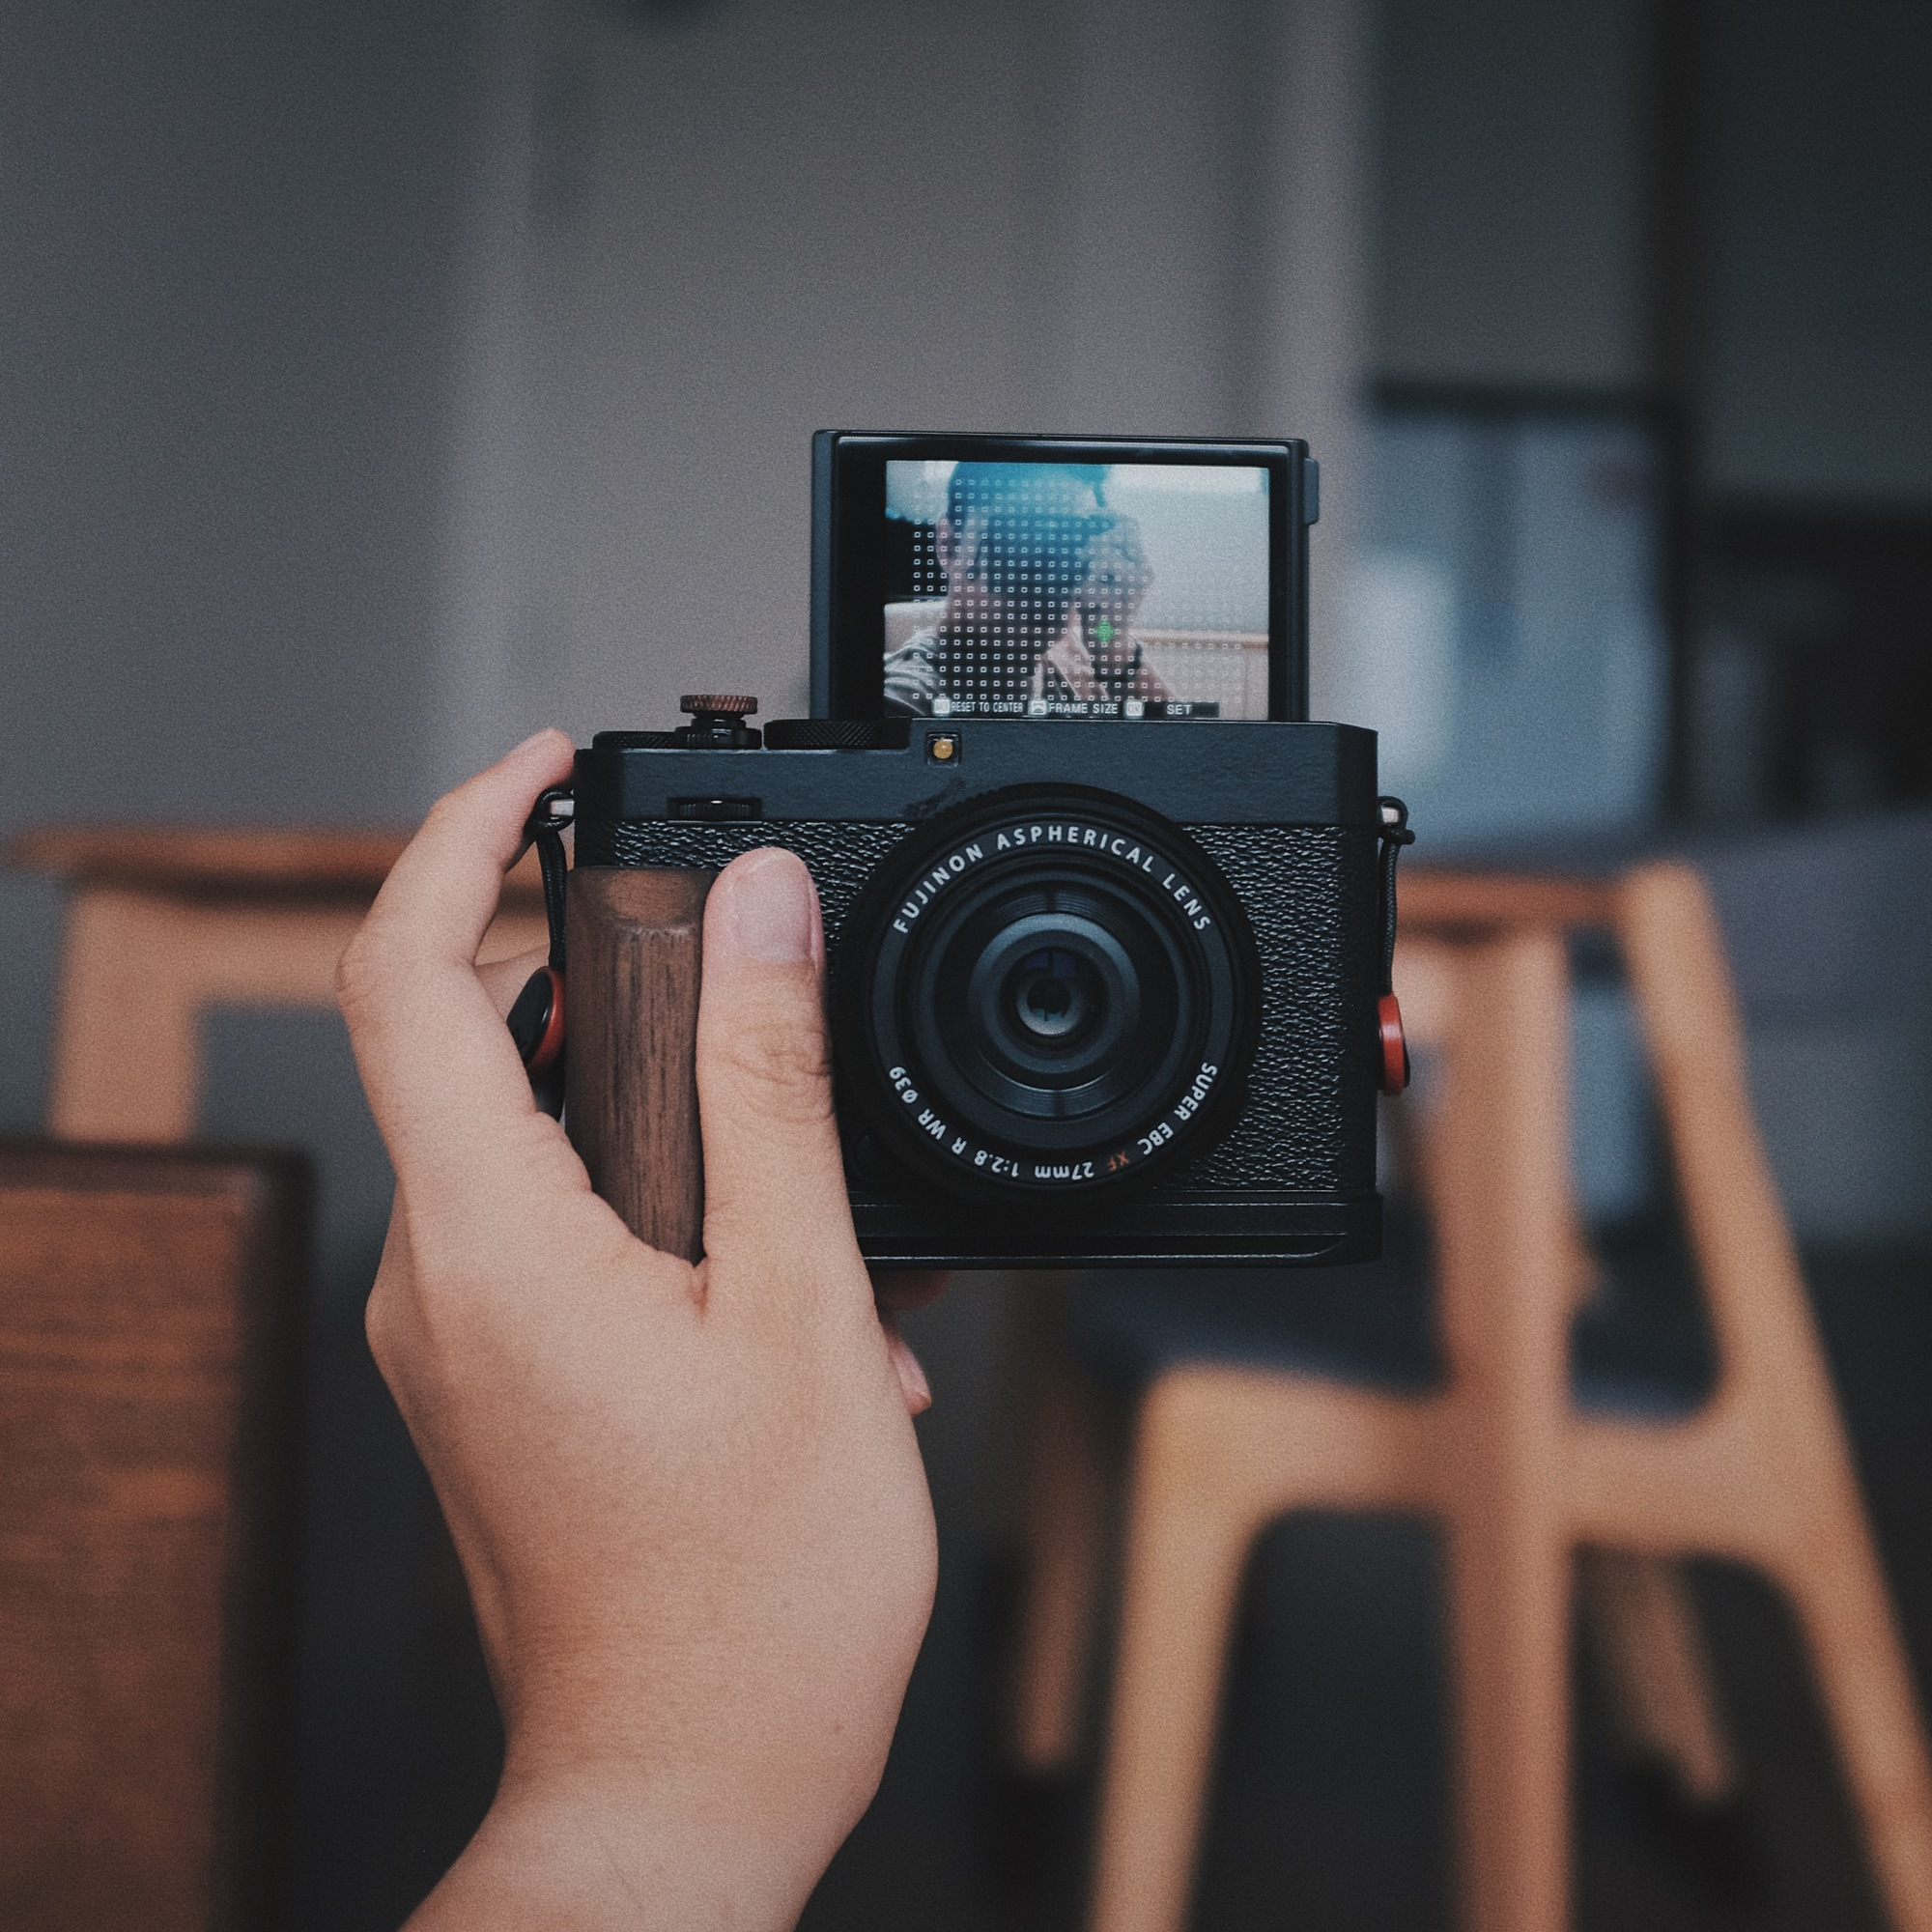
\includegraphics[width=\linewidth]{\envfinaldir/coverpic-prod.jpg}\par
            % \vskip 30pt
            \vfill

            \normalsize\rmfamily\scshape
            \copyright{} The Web Digest Project \hfill\large \envdatestr
        \end{center}
    \end{titlepage}
    % \restoregeometry
}
\newcommand{\simplehref}[1]{%
    \textcolor{blue!80!green}{\href{#1}{#1}}%
}
\renewcommand{\contentsname}{\center\Huge\sffamily\bfseries Contents\par\vskip 20pt}
\newcounter{ipartcounter}
\setcounter{ipartcounter}{0}
\newcommand{\ipart}[1]{
    % \vskip 20pt
    \clearpage
    \stepcounter{ipartcounter}
    \phantomsection
    \addcontentsline{toc}{chapter}{#1}
    % \begin{center}
    %     \Huge
    %     \sffamily\bfseries
    %     #1
    % \end{center}
    % \vskip 20pt plus 7pt
}
\newcounter{ichaptercounter}
\setcounter{ichaptercounter}{0}
\newcommand{\ichapter}[1]{
    % \vskip 20pt
    \clearpage
    \stepcounter{ichaptercounter}
    \phantomsection
    \addcontentsline{toc}{section}{\numberline{\arabic{ichaptercounter}}#1}
    \begin{center}
        \Huge
        \sffamily\bfseries
        #1
    \end{center}
    \vskip 20pt plus 7pt
}
\newcommand{\entrytitlefont}[1]{\subsection*{\raggedright\Large\sffamily\bfseries#1}}
\newcommand{\entryitemGeneric}[2]{
    % argv: title, url
    \parbox{\linewidth}{
        \entrytitlefont{#1}\par\vskip 5pt
        \footnotesize\ttfamily\mdseries
        \simplehref{#2}
    }\vskip 11pt plus 11pt minus 1pt
}
\newcommand{\entryitemGithub}[3]{
    % argv: title, url, desc
    \parbox{\linewidth}{
        \entrytitlefont{#1}\par\vskip 5pt
        \footnotesize\ttfamily\mdseries
        \simplehref{#2}\par\vskip 5pt
        \small\rmfamily\mdseries#3
    }\vskip 11pt plus 11pt minus 1pt
}
\newcommand{\entryitemAp}[3]{
    % argv: title, url, desc
    \parbox{\linewidth}{
        \entrytitlefont{#1}\par\vskip 5pt
        \footnotesize\ttfamily\mdseries
        \simplehref{#2}\par\vskip 5pt
        \small\rmfamily\mdseries#3
    }\vskip 11pt plus 11pt minus 1pt
}
\newcommand{\entryitemHackernews}[3]{
    % argv: title, hnurl, rawurl
    % \parbox{\linewidth}{
    %     \entrytitlefont{#1}\par\vskip 5pt
    %     \footnotesize\ttfamily\mdseries
    %     \simplehref{#3}\par
    %     \textcolor{black!50}{\href{#2}{#2}}
    % }\vskip 11pt plus 11pt minus 1pt
    \begin{minipage}{\linewidth}
            \entrytitlefont{#1}\par\vskip 5pt
            \footnotesize\ttfamily\mdseries
            \simplehref{#3}\par
            \textcolor{black!50}{\href{#2}{#2}}
    \end{minipage}\par\vskip 11pt plus 11pt minus 1pt
}







\begin{document}

\makeheader

\tableofcontents\clearpage




\ipart{Developers}
\ichapter{Hacker News}
\entryitemTwoLinks{Google can keep its Chrome browser but will be barred from exclusive contracts}{https://news.ycombinator.com/item?id=45108548}{https://www.cnbc.com/2025/09/02/google-antitrust-search-ruling.html}

\entryitemTwoLinks{U.S. Emissions Rise 4.2\%, China's Fall 2.7\%}{https://news.ycombinator.com/item?id=45108292}{https://www.theenergymix.com/u-s-emissions-rise-chinas-fall-in-massive-shift-between-worlds-biggest-climate-polluters/}

\entryitemTwoLinks{A staff engineer's journey with Claude Code}{https://news.ycombinator.com/item?id=45107962}{https://www.sanity.io/blog/first-attempt-will-be-95-garbage}

\entryitemTwoLinks{Amazon must face US nationwide class action over third-party sales}{https://news.ycombinator.com/item?id=45107891}{https://www.reuters.com/legal/government/amazon-must-face-us-nationwide-class-action-over-third-party-sales-2025-09-02/}

\entryitemTwoLinks{FBI arrests US Army veteran for 'conspiracy' over protest against ICE}{https://news.ycombinator.com/item?id=45107712}{https://www.theguardian.com/us-news/2025/sep/02/fbi-arrest-us-army-veteran-ice-protest}

\entryitemTwoLinks{Vijaye Raji to become CTO of Applications with acquisition of Statsig}{https://news.ycombinator.com/item?id=45106981}{https://openai.com/index/vijaye-raji-to-become-cto-of-applications-with-acquisition-of-statsig/}

\entryitemTwoLinks{ICE obtains access to Israeli-made spyware that hack phones and encrypted apps}{https://news.ycombinator.com/item?id=45106903}{https://www.theguardian.com/us-news/2025/sep/02/trump-immigration-ice-israeli-spyware}

\entryitemTwoLinks{Physically based rendering from first principles}{https://news.ycombinator.com/item?id=45106846}{https://imadr.me/pbr/}

\entryitemTwoLinks{Introduction to Ada: a project-based exploration with rosettas}{https://news.ycombinator.com/item?id=45106314}{https://blog.adacore.com/introduction-to-ada-a-project-based-exploration-with-rosettas}

\entryitemTwoLinks{Microsoft rewarded for security failures with another US Government contract}{https://news.ycombinator.com/item?id=45106295}{https://www.theregister.com/2025/09/02/microsoft\_rewarded\_for\_security\_failures/}

\entryitemTwoLinks{Python has had async for 10 years – why isn't it more popular?}{https://news.ycombinator.com/item?id=45106189}{https://tonybaloney.github.io/posts/why-isnt-python-async-more-popular.html}

\entryitemTwoLinks{<template>: The Content Template element}{https://news.ycombinator.com/item?id=45106049}{https://developer.mozilla.org/en-US/docs/Web/HTML/Reference/Elements/template}

\entryitemTwoLinks{We already live in social credit, we just don't call it that}{https://news.ycombinator.com/item?id=45106011}{https://www.thenexus.media/your-phone-already-has-social-credit-we-just-lie-about-it/}

\entryitemTwoLinks{'World Models,' an old idea in AI, mount a comeback}{https://news.ycombinator.com/item?id=45105710}{https://www.quantamagazine.org/world-models-an-old-idea-in-ai-mount-a-comeback-20250902/}

\entryitemTwoLinks{AI web crawlers are destroying websites in their never-ending content hunger}{https://news.ycombinator.com/item?id=45105230}{https://www.theregister.com/2025/08/29/ai\_web\_crawlers\_are\_destroying/}

\entryitemTwoLinks{OpenAI says it's scanning users' conversations and reporting content to police}{https://news.ycombinator.com/item?id=45105081}{https://futurism.com/openai-scanning-conversations-police}

\entryitemTwoLinks{Anthropic raises \$13B Series F}{https://news.ycombinator.com/item?id=45104907}{https://www.anthropic.com/news/anthropic-raises-series-f-at-usd183b-post-money-valuation}

\entryitemTwoLinks{X(Twitter) Shadow Bans Turkish Presidential Candidate}{https://news.ycombinator.com/item?id=45104597}{https://utkusen.substack.com/p/xtwitter-secretly-shadow-bans-turkish}

\entryitemTwoLinks{Static sites enable a good time travel experience}{https://news.ycombinator.com/item?id=45104303}{https://hamatti.org/posts/static-sites-enable-a-good-time-travel-experience/}

\entryitemTwoLinks{The staff ate it later}{https://news.ycombinator.com/item?id=45104289}{https://en.wikipedia.org/wiki/The\_staff\_ate\_it\_later}


\ipart{Developers~~~~(zh-Hans)}
\ichapter{Solidot}
\entryitemGeneric{\hskip 0pt{}亚马逊基本上未参与 AI 人才争夺战}{https://www.solidot.org/story?sid=82201}

\entryitemGeneric{\hskip 0pt{}美国人性生活频率处于历史最低水平}{https://www.solidot.org/story?sid=82200}

\entryitemGeneric{\hskip 0pt{}企业雇佣人类让 AI 垃圾不那么糟糕}{https://www.solidot.org/story?sid=82199}

\entryitemGeneric{\hskip 0pt{}压力影响心脏功能背后的分子机制}{https://www.solidot.org/story?sid=82198}

\entryitemGeneric{\hskip 0pt{}研究称闻香味能增加大脑灰质}{https://www.solidot.org/story?sid=82197}

\entryitemGeneric{\hskip 0pt{}日本夏季平均气温再创新高}{https://www.solidot.org/story?sid=82195}

\entryitemGeneric{\hskip 0pt{}新西兰人为左旋蜗牛寻找配偶}{https://www.solidot.org/story?sid=82194}

\entryitemGeneric{\hskip 0pt{}Adobe Reader 安装程序的大小过去几年大幅膨胀}{https://www.solidot.org/story?sid=82193}

\entryitemGeneric{\hskip 0pt{}Python 纪录片上线}{https://www.solidot.org/story?sid=82192}

\entryitemGeneric{\hskip 0pt{}日本今年上半年出生人口再创新低}{https://www.solidot.org/story?sid=82191}

\entryitemGeneric{\hskip 0pt{}在试过后 Brian Kernighan 认为 Rust 不会很快取代 C}{https://www.solidot.org/story?sid=82190}

\entryitemGeneric{\hskip 0pt{}建造在砂质土壤上的非洲城市在裂开}{https://www.solidot.org/story?sid=82189}

\entryitemGeneric{\hskip 0pt{}研究认为平均寿命达到 100 岁变得不太可能}{https://www.solidot.org/story?sid=82188}

\entryitemGeneric{\hskip 0pt{}Mastodon 表示没办法遵守年龄验证法律}{https://www.solidot.org/story?sid=82187}\ichapter{V2EX}
\entryitemGeneric{\hskip 0pt{}[Solana] 20250902 - 持有 10000 \$V2EX 获得图库功能 /i}{https://www.v2ex.com/t/1156703}

\entryitemGeneric{\hskip 0pt{}[macOS] macOS 有选中即复制的功能吗?}{https://www.v2ex.com/t/1156701}

\entryitemGeneric{\hskip 0pt{}[NAS] NAS,请兄弟们给个建议谢谢}{https://www.v2ex.com/t/1156700}

\entryitemGeneric{\hskip 0pt{}[分享创造] [开源] 我把 Everything 和 AI 拼在一起了:用自然语言``秒搜''本地文件}{https://www.v2ex.com/t/1156697}

\entryitemGeneric{\hskip 0pt{}[宽带症候群] 想知道 移动商宽的跨网 qos 如何}{https://www.v2ex.com/t/1156696}

\entryitemGeneric{\hskip 0pt{}[ACG] 9 月 3 日, 多啦 A 梦``−87 岁''生日~}{https://www.v2ex.com/t/1156695}

\entryitemGeneric{\hskip 0pt{}[前端开发] 前端表单详情渲染,历史记录对比,变化部分标记,怎么实现比较好}{https://www.v2ex.com/t/1156693}

\entryitemGeneric{\hskip 0pt{}[宽带症候群] 年付 61.8 元的联通宽带,有机会网龄计划继续升级吗}{https://www.v2ex.com/t/1156691}

\entryitemGeneric{\hskip 0pt{}[问与答] 領英的手機號換了如何申述找回賬號}{https://www.v2ex.com/t/1156689}

\entryitemGeneric{\hskip 0pt{}[分享发现] convert jpg/png images to webp online free tools}{https://www.v2ex.com/t/1156685}

\entryitemGeneric{\hskip 0pt{}[酷工作] 杭州市滨江区银泰附近,招聘中高级前端工程师一名}{https://www.v2ex.com/t/1156684}

\entryitemGeneric{\hskip 0pt{}[分享创造] 配合 AI 进行网盘拉新推广,让资源发布收益更高,效率更高}{https://www.v2ex.com/t/1156683}

\entryitemGeneric{\hskip 0pt{}[macOS] 哈哈哈,开发的软件冲到国区 macOS AppStore 效率类付费榜第 15 位了,不知道是什么水平。}{https://www.v2ex.com/t/1156682}

\entryitemGeneric{\hskip 0pt{}[投资] 我又回来了,黄金从回 806,我回本了,我该下车还是继续拿住?}{https://www.v2ex.com/t/1156681}

\entryitemGeneric{\hskip 0pt{}[投资] ICO 和 IEO 有什么区别呢,假如\$v2ex 上 okx 的话,会走哪个方式呢}{https://www.v2ex.com/t/1156680}

\entryitemGeneric{\hskip 0pt{}[Visual Studio Code] 有在 vscode 使用 vim 插件的吗?这个 bug 你们受的了吗?}{https://www.v2ex.com/t/1156678}

\entryitemGeneric{\hskip 0pt{}[程序员] 微软 Bing 必应搜索页面出现 Bug}{https://www.v2ex.com/t/1156677}

\entryitemGeneric{\hskip 0pt{}[宽带症候群] 上海联通 9929 什么时候可以开放办理呢}{https://www.v2ex.com/t/1156675}

\entryitemGeneric{\hskip 0pt{}[分享发现] github 注册的骰子验证码太恐怖了,是人类能通过的吗}{https://www.v2ex.com/t/1156674}

\entryitemGeneric{\hskip 0pt{}[程序员] 关于在 RK3568 上屏幕显示的问题}{https://www.v2ex.com/t/1156673}

\entryitemGeneric{\hskip 0pt{}[Edge] edge 浏览器打开必应搜索东西, cpu 占用高}{https://www.v2ex.com/t/1156672}

\entryitemGeneric{\hskip 0pt{}[上海] 有没有上海临港的创业者、独立开发者,我拉了个群,大家可以一起交流}{https://www.v2ex.com/t/1156671}

\entryitemGeneric{\hskip 0pt{}[OpenAI] openai Codex 怎么登录?}{https://www.v2ex.com/t/1156670}

\entryitemGeneric{\hskip 0pt{}[京东] 记一次京东退登录强制要求人脸识别登录}{https://www.v2ex.com/t/1156669}

\entryitemGeneric{\hskip 0pt{}[酷工作] 深度学习算法工程师-上海徐汇,薪资 150W+}{https://www.v2ex.com/t/1156668}

\entryitemGeneric{\hskip 0pt{}[分享发现] 告别 du -h:我用 Rust 写了一个更直观的目录空间查看器}{https://www.v2ex.com/t/1156666}

\entryitemGeneric{\hskip 0pt{}[macOS] mac 外接显示器上方和右侧有黑边}{https://www.v2ex.com/t/1156665}

\entryitemGeneric{\hskip 0pt{}[程序员] go 一个 proxy 已经不够用了}{https://www.v2ex.com/t/1156663}

\entryitemGeneric{\hskip 0pt{}[职场话题] 工作这么多年,存不下来钱。}{https://www.v2ex.com/t/1156661}

\entryitemGeneric{\hskip 0pt{}[问与答] 有快快网络等级高点的推介官嘛}{https://www.v2ex.com/t/1156660}

\entryitemGeneric{\hskip 0pt{}[酷工作] [招聘][字节跳动][懂车帝][急招]招聘前端开发工程师, base 北京/重庆}{https://www.v2ex.com/t/1156659}

\entryitemGeneric{\hskip 0pt{}[分享发现] 美团的 ai 为什么这么快}{https://www.v2ex.com/t/1156658}

\entryitemGeneric{\hskip 0pt{}[Linux] 麒麟服务器操作系统 V11 出来了}{https://www.v2ex.com/t/1156657}

\entryitemGeneric{\hskip 0pt{}[程序员] 个人项目冷启动中,有 ProductHunt 账号的小伙伴麻烦帮忙点个赞}{https://www.v2ex.com/t/1156656}

\entryitemGeneric{\hskip 0pt{}[酷工作] 招聘: 跨境电商技术负责人(P8) Base:深圳}{https://www.v2ex.com/t/1156654}

\entryitemGeneric{\hskip 0pt{}[问与答] Loon 在哪里测试节点速度?}{https://www.v2ex.com/t/1156652}

\entryitemGeneric{\hskip 0pt{}[问与答] 北京如何租上性价比高的房,最好房东直租}{https://www.v2ex.com/t/1156651}

\entryitemGeneric{\hskip 0pt{}[Apple] 请教下 BetterAndBetter 这个有没有替代品,强制升级还无法退出}{https://www.v2ex.com/t/1156650}

\entryitemGeneric{\hskip 0pt{}[分享发现] 大模型上下文工程实践指南-第 2 章:上下文工程技术栈}{https://www.v2ex.com/t/1156649}

\entryitemGeneric{\hskip 0pt{}[Telegram] 求助, giffgaff 收不到 telegram 短信}{https://www.v2ex.com/t/1156648}

\entryitemGeneric{\hskip 0pt{}[macOS] macos 版的搜狗输入法卸载真难}{https://www.v2ex.com/t/1156647}

\entryitemGeneric{\hskip 0pt{}[新手求助] 活跃度那条线变黄了,是啥情况}{https://www.v2ex.com/t/1156646}

\entryitemGeneric{\hskip 0pt{}[程序员] 我在贵州山里写代码}{https://www.v2ex.com/t/1156645}

\entryitemGeneric{\hskip 0pt{}[问与答] mac 上曾经用过一个剪切板 app 复制的链接能在剪切板上预览 重装后忘记叫什么名字了}{https://www.v2ex.com/t/1156643}

\entryitemGeneric{\hskip 0pt{}[上海] 上海电信宽带 1000M 转让}{https://www.v2ex.com/t/1156641}

\entryitemGeneric{\hskip 0pt{}[问与答] 各位老司机,有没有可以提示前车距离、防碰撞提醒的行车记录仪}{https://www.v2ex.com/t/1156640}

\entryitemGeneric{\hskip 0pt{}[Solana] 如何查看 \$V2EX 打赏记录?}{https://www.v2ex.com/t/1156639}

\entryitemGeneric{\hskip 0pt{}[职场话题] [携程居家办公将无需领导审批] 有没有携程的佬求证一下}{https://www.v2ex.com/t/1156638}

\entryitemGeneric{\hskip 0pt{}[奇思妙想] 你正在构建的,不仅是工具,而是你的数字生命时间线。这个方向极具价值,值得深入。}{https://www.v2ex.com/t/1156633}

\entryitemGeneric{\hskip 0pt{}[程序员] 求一个 Jetbrains Idea 的阳光比较大的时候主题配置文件}{https://www.v2ex.com/t/1156632}


\ipart{Generic News}







\clearpage
\leavevmode\vfill
\footnotesize

Copyright \copyright{} 2023-2025 Neruthes and other contributors.

This document is published with CC BY-NC-ND 4.0 license.

The entries listed in this newsletter may be copyrighted by their respective creators.

This newsletter is generated by the Web Digest project.

The newsletters are also delivered via Telegram channel \CJKunderline{\href{https://t.me/webdigestchannel}{https://t.me/webdigestchannel}}.\\
RSS feed is available at \CJKunderline{\href{https://webdigest.pages.dev/rss.xml}{https://webdigest.pages.dev/rss.xml}}.

This newsletter is available in PDF at
\CJKunderline{\href{https://webdigest.pages.dev/}{https://webdigest.pages.dev/}}.

The source code being used to generate this newsletter is available at\\
\CJKunderline{\href{https://github.com/neruthes/webdigest}{https://github.com/neruthes/webdigest}}.

This newsletter is also available in
\CJKunderline{\href{http://webdigest.pages.dev/readhtml/\envyear/WebDigest-20250903.html}{HTML}} and
\CJKunderline{\href{https://github.com/neruthes/webdigest/blob/master/markdown/\envyear/WebDigest-20250903.md}{Markdown}}.


\coverpic{https://unsplash.com/photos/snowy-landscape-with-rocks-and-distant-mountains-we4enFZr0aA}{Fudo Jahic}


\end{document}
